../../hw03/report/pcsmacros.tex
\include{pythonlisting}

\title[]{Extended imaging and tomography under two-way operators}
\subtitle{}
\author[]{Esteban D\'{i}az}
\date{}
\logo{}



\huge

\def\big#1{\begin{center} \LARGE \textbf{#1} \end{center}}
\def\cen#1{\begin{center}        \textbf{#1} \end{center}}


\tikzstyle{arrow}=[draw, -latex] 
\tikzstyle{rarrow}=[arrow,line width=.8mm,draw=red, fill=red]
\tikzstyle{karrow}=[arrow,scale=.5,line width=.8mm,draw=black, fill=black]
\tikzstyle{RectObject}=[rectangle,fill=white,draw,line width=0.5mm]


% ------------------------------------------------------------
\mode<beamer> { \cwpcover }

\setbeamertemplate{footline}[frame number] 



\inputdir{XFig}


\begin{frame}
\vspace{-2cm}
  \plot{objectiveFWD}{width=\textwidth}{}
\end{frame}
\begin{frame}
\vspace{-2cm}
  \plot{objectiveSCT}{width=\textwidth}{}
\end{frame}


\begin{frame}
\vspace{-2cm}
  \plot{swfl}{width=\textwidth}{}
\end{frame}



\begin{frame}
\vspace{-2cm}
  \plot{rwfl}{width=\textwidth}{}
\end{frame}

\begin{frame}
\vspace{-2cm}
  \plot{objectiveIMG}{width=\textwidth}{}
\end{frame}


\begin{frame}
\vspace{-2cm}
  \plot{SCT}{width=\textwidth}{}
\end{frame}




\begin{frame}
\vspace{-2cm}
  \plot{objectiveTOM}{width=\textwidth}{}
\end{frame}




\begin{frame} \frametitle{first comps/ MSc Thesis}
  \Large
  \begin{enumerate}
    \item understanding rtm backscattering: noise or signal?
    \item wavefield tomography using rtm backscattering
  \end{enumerate} 
\end{frame}


\begin{frame} \frametitle{first comps/ MSc Thesis}
  \Large

  \begin{enumerate}
    \item understanding rtm backscattering: noise or signal? (published)
    \item wavefield tomography using rtm backscattering (published)
  \end{enumerate} 
\end{frame}


\begin{frame} \frametitle{PhD thesis}
  \Large

  \begin{enumerate}
    \item CIP wavefield tomography with illumination compensation
    \item seismic tomography using local correlation functions
    \item extended imaging analysis using Marchenko wavefields
    \item wavefield tomography using multiple scattered waves
  \end{enumerate} 
\end{frame}


\begin{frame} \frametitle{PhD thesis}
  \Large

  \begin{enumerate}
    \item CIP wavefield tomography with illumination compensation
    \item \gray{seismic tomography using local correlation functions}
    \item \gray{extended imaging analysis using Marchenko wavefields}
    \item \gray{wavefield tomography using multiple scattered waves}
  \end{enumerate} 
\end{frame}







\begin{frame}
  \[
     R(\xx,\hh,\tau) =
     \sum_{t} u_s(\xx+\hh,t+\tau) u_r(\xx-\hh,t-\tau)
  \]
\sep  
  \itab{$u_s$: source wavefield} \\ 
  \itab{$u_r$: receiver wavefield}\\
  \itab{$\hh,\tau$: space and time-lags}  
\end{frame}

\begin{frame}
  \[
     R(\red{\xx},\hh,\tau) =
     \sum_{t} u_s(\red{\xx}+\hh,t+\tau) u_r(\red{\xx}-\hh,t-\tau)
  \]
\sep  
  \itab{$u_s$: source wavefield} \\ 
  \itab{$u_r$: receiver wavefield}\\
  \itab{$\hh,\tau$: space and time-lags}  

\end{frame}

\begin{frame}
  \[
     R(\xx_c,\hh,\tau) =
     \sum_{t} u_s(\xx_c+\hh,t+\tau) u_r(\xx_c-\hh,t-\tau)
  \]
\sep  
  \itab{$u_s$: source wavefield}\\
  \itab{$u_r$: receiver wavefield}\\
  \itab{$\hh,\tau$: space and time-lags}  
\end{frame}




\begin{frame}
  \[
  J(\m) = \ltnorm{P(\hh,\tau) R(\xx_c,\hh,\tau)}
  \]
\sep
  \itab{$P(\hh,\tau):$ penalty operator}\\
  \itab{$\m$: model parameter}
  \begin{flushright}
  (Yang, 2013)
  \end{flushright}
\end{frame}



\begin{frame}
  \[
  J(\m) = -\ltnorm{H(\hh,\tau) R(\xx_c,\hh,\tau)}
  \]
\sep
  \itab{$H(\hh,\tau):$ highlight operator}\\
  \itab{$\m$: model parameter}
  \begin{flushright}
  \end{flushright}
\end{frame}



\inputdir{workshop}


\begin{frame}
  \vspace{.63cm}
    \begin{flushleft}
      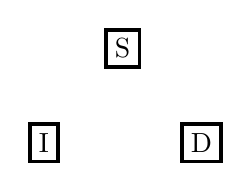
\begin{tikzpicture}
        \path (0,0)  node[RectObject] (x) {{\red S}}; 
        \path (1.,-1.2) node[RectObject] (y) {D};
        \path (-1,-1.2)  node[RectObject] (z) {I};
      \end{tikzpicture}
    \end{flushleft}
  \vspace{-1cm}
 \plot{image-wtomo-cip}{width=\textwidth}{}
\end{frame}




\begin{frame}
  \vspace{.63cm}
    \begin{flushleft}
      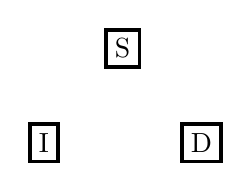
\begin{tikzpicture}
        \path (0,0)  node[RectObject] (x) {{\red S}}; 
        \path (1.,-1.2) node[RectObject] (y) {D};
        \path (-1,-1.2)  node[RectObject] (z) {I};
      \end{tikzpicture}
    \end{flushleft}
  \vspace{-1cm}
 \plot{image-winit}{width=\textwidth}{}
\end{frame}


\begin{frame}
  \vspace{.63cm}
    \begin{flushleft}
      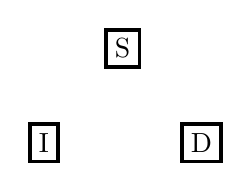
\begin{tikzpicture}
        \path (0,0)  node[RectObject] (x) {S}; 
        \path (1.,-1.2) node[RectObject] (y) {D};
        \path (-1,-1.2)  node[RectObject] (z) {{\red I}};
      \end{tikzpicture}
    \end{flushleft}
  \vspace{-1cm}
 \plot{image-wtomo}{width=\textwidth}{}
\end{frame}

\begin{frame}
  \vspace{.63cm}
    \begin{flushleft}
      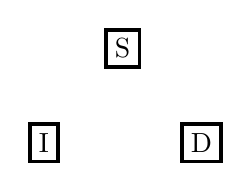
\begin{tikzpicture}
        \path (0,0)  node[RectObject] (x) {S}; 
        \path (1.,-1.2) node[RectObject] (y) {{\red D}};
        \path (-1,-1.2)  node[RectObject] (z) {I};
      \end{tikzpicture}
    \end{flushleft}
  \vspace{-1cm}
 \plot{image-wfwi}{width=\textwidth}{}
\end{frame}











\begin{frame} \frametitle{PhD thesis}
  \Large

  \begin{enumerate}
    \item  \gray{CIP wavefield tomography with illumination compensation}
    \item seismic tomography using local correlation functions
    \item \gray{extended imaging analysis using Marchenko wavefields}
    \item \gray{wavefield tomography using multiple scattered waves}
  \end{enumerate} 
\end{frame}



%\begin{frame}
%  Global correlation
%\[
%  c(\tau) =  \int f\lp t'-\frac{\tau}{2}\rp g\lp t'+\frac{\tau}{2}\rp dt'
%\]
%\[
%  {\bf c} = \mathbf{C} {\bf f}
%\]
%\end{frame}
%\begin{frame}
%  Local correlation
%\[
%  c(t,\tau) = 
%  \int w(t-t') f\lp t'-\frac{\tau}{2}\rp g\lp t'+\frac{\tau}{2} \rp dt'
%\]
%\[
% w (t-t') \equiv e^{-\tau^2/4\sigma^2}e^{-(t-t')^2/\sigma^2}
%\]
%\end{frame}
%
%\begin{frame}
%  Local correlation
%\[
%  c(t,\tau) = 
%  \int w(t-t') f \lp t'-\frac{\tau}{2}\rp g\lp t'+\frac{\tau}{2} \rp dt'
%\]
%\[
% \red {w (t-t') \equiv e^{-\tau^2/4\sigma^2}e^{-(t-t')^2/\sigma^2}}
%\]
%\end{frame}
%
%\begin{frame}
%  Local correlation
%\[
%  c(t,\tau) = 
%  \int w(t-t') f \lp t'-\frac{\tau}{2}\rp g\lp t'+\frac{\tau}{2}\rp dt'
%\]
%\[
%  {\bf c} = \mathbf{C} {\bf f}
%\]
%\end{frame}
%
%
%\begin{frame}
%  \begin{columns}
%    \column{0.5\textwidth}
%    \vfill
%      \center
%      Local Correlation 
%        \[
%        {\bf C} = {\bf G S}
%        \]
%    \vfill
%    \pause
%    \column{0.5\textwidth}
%    \vfill
%      \center
%      Local Convolution
%        \[
%        {\bf C}^\top = {\bf S}^\top {\bf G}
%        \]
%    \vfill
%  \end{columns}
%\sep
%\itab{$\bf G$: Gaussian filter matrix}\\
%\itab{$\bf S$: matrix with shifted versions of $\bf g$}
%\end{frame}
%





\inputdir{lcorr}




\begin{frame}
  \plot{f}{}{\klabel{10}{30}{${ f(t)}$}}
\end{frame}

\begin{frame}
  \plot{g}{}{\klabel{10}{30}{${ g(t)}$}}
\end{frame}

\begin{frame}
  \plot{corr}{}{\wlabel{20}{5}{$f\star g,\sigma=0.04$s}}
\end{frame}

\begin{frame}
  \plot{gcorr}{}
    {\wlabel{20}{5}{$f\star g,\sigma\rightarrow \infty$}}
\end{frame}

%\begin{frame}
%  \big{examples}
%\end{frame}
%
%\inputdir{example}
%
%
%\begin{frame}
%  \plot{vel-neg}{}{\klabel{72}{30}{slow}}
%\end{frame}
%
%\begin{frame}
%  \plot{vel-zer}{}{\klabel{72}{30}{correct}}
%\end{frame}
%
%\begin{frame}
%  \plot{vel-pos}{}{\klabel{72}{30}{fast}}
%\end{frame}
%
%\begin{frame}
%  \plot{data-comp}{}{}
%\end{frame}
%
%\begin{frame}
%  \plot{gr-penaltyBP-global-vel-neg}{}
%    {\klabel{15}{-3}{$\sigma\rightarrow \infty$}
%     \klabel{70}{-3}{slow}
%      }
%\end{frame}
%\begin{frame}
%  \plot{gr-penaltyBP-global-vel-zer}{}
%    {\klabel{15}{-3}{$\sigma\rightarrow \infty$}
%     \klabel{70}{-3}{correct}
%      }
%\end{frame}
%\begin{frame}
%  \plot{gr-penaltyBP-global-vel-pos}{}
%    {\klabel{15}{-3}{$\sigma\rightarrow \infty$}
%     \klabel{70}{-3}{fast}
%      }
%\end{frame}
%
%
%\begin{frame}
%  \plot{gr-penaltyBP-local-vel-neg}{}
%    {\klabel{15}{-3}{$\sigma=0.1s$}
%     \klabel{70}{-3}{slow}
%      }
%\end{frame}
%\begin{frame}
%  \plot{gr-penaltyBP-local-vel-zer}{}
%    {\klabel{15}{-3}{$\sigma=0.1s$}
%     \klabel{70}{-3}{correct}
%      }
%\end{frame}
%\begin{frame}
%  \plot{gr-penaltyBP-local-vel-pos}{}
%    {\klabel{15}{-3}{$\sigma=0.1s$}
%     \klabel{70}{-3}{fast}
%      }
%\end{frame}
%\begin{frame}
%  \plot{gr-penaltyBP-global-vel-pos}{}
%    {\klabel{15}{-3}{$\sigma\rightarrow \infty$}
%     \klabel{70}{-3}{fast}
%      }
%\end{frame}
%
%
%\begin{frame}
%  \plot{gr-penaltyBP-local-vel-neg}{}
%    {\klabel{15}{-3}{$\sigma=0.1s$}
%     \klabel{70}{-3}{slow}
%      }
%\end{frame}
%\begin{frame}
%  \plot{gr-penaltyBP-global-vel-neg}{}
%    {\klabel{15}{-3}{$\sigma\rightarrow \infty$}
%     \klabel{70}{-3}{slow}
%      }
%\end{frame}

\begin{frame} \frametitle{PhD thesis}
  \Large

  \begin{enumerate}
    \item \gray{CIP wavefield tomography with illumination compensation}
    \item \gray{seismic tomography using local correlation functions}
    \item {extended imaging analysis using Marchenko wavefields}
    \item \gray{wavefield tomography using multiple scattered waves}
  \end{enumerate} 
\end{frame}

\inputdir{kernels}






\begin{frame}
  \plot{ss-xx-kernel-fsm}{}{}
\end{frame}
\begin{frame}
  \plot{ss-xx-kernel-f}{}{}
\end{frame}





\inputdir{XFig}



\begin{frame}
  \plot{f-3}{width=0.7\textwidth}{\klabellarge{45}{-5}{(after Singh et al., 2015)}}
\end{frame}

\begin{frame}
  \plot{f-2}{width=0.7\textwidth}{\klabellarge{45}{-5}{(after Singh et al., 2015)}}
\end{frame}

\begin{frame}
  \plot{f-1}{width=0.7\textwidth}{\klabellarge{45}{-5}{(after Singh et al., 2015)}}
\end{frame}

\begin{frame}
  \plot{f-0}{width=0.7\textwidth}{\klabellarge{45}{-5}{(after Singh et al., 2015)}}
\end{frame}

\begin{frame}
  \plot{g+1}{width=0.7\textwidth}{\klabellarge{45}{-5}{(after Singh et al., 2015)}}
\end{frame}

\begin{frame}
  \plot{g+2}{width=0.7\textwidth}{\klabellarge{45}{-5}{(after Singh et al., 2015)}}
\end{frame}

\inputdir{forMarchenko}
\begin{frame}
  \plot{ro}{}{}
\end{frame}

\begin{frame}
  \plot{shot250}{}{}
\end{frame}


\begin{frame}
\begin{columns}
  \column{0.5\textwidth}
    \plot{Gp_perc_100_t-0000}{}{\klabellarge{45}{-5}{$G^+$}}
  \column{0.5\textwidth}
    \plot{Gm_perc_100_t-0000}{}{\klabellarge{-20}{-15}{$t=0.0s$}\klabellarge{45}{-5}{$G^-$}}
\end{columns}
\end{frame}


\begin{frame}
\begin{columns}
  \column{0.5\textwidth}
    \plot{Gp_perc_100_t-0001}{}{\klabellarge{45}{-5}{$G^+$}}
  \column{0.5\textwidth}
    \plot{Gm_perc_100_t-0001}{}{\klabellarge{-20}{-15}{$t=0.1s$}\klabellarge{45}{-5}{$G^-$}}
\end{columns}
\end{frame}

\begin{frame}
\begin{columns}
  \column{0.5\textwidth}
    \plot{Gp_perc_100_t-0002}{}{\klabellarge{45}{-5}{$G^+$}}
  \column{0.5\textwidth}
    \plot{Gm_perc_100_t-0002}{}{\klabellarge{-20}{-15}{$t=0.2s$}\klabellarge{45}{-5}{$G^-$}}
\end{columns}
\end{frame}

\begin{frame}
\begin{columns}
  \column{0.5\textwidth}
    \plot{Gp_perc_100_t-0003}{}{\klabellarge{45}{-5}{$G^+$}}
  \column{0.5\textwidth}
    \plot{Gm_perc_100_t-0003}{}{\klabellarge{-20}{-15}{$t=0.3s$}\klabellarge{45}{-5}{$G^-$}}
\end{columns}
\end{frame}

\begin{frame}
\begin{columns}
  \column{0.5\textwidth}
    \plot{Gp_perc_100_t-0004}{}{\klabellarge{45}{-5}{$G^+$}}
  \column{0.5\textwidth}
    \plot{Gm_perc_100_t-0004}{}{\klabellarge{-20}{-15}{$t=0.4s$}\klabellarge{45}{-5}{$G^-$}}
\end{columns}
\end{frame}

\begin{frame}
\begin{columns}
  \column{0.5\textwidth}
    \plot{Gp_perc_100_t-0005}{}{\klabellarge{45}{-5}{$G^+$}}
  \column{0.5\textwidth}
    \plot{Gm_perc_100_t-0005}{}{\klabellarge{-20}{-15}{$t=0.5s$}\klabellarge{45}{-5}{$G^-$}}
\end{columns}
\end{frame}


\begin{frame}
\begin{columns}
  \column{0.5\textwidth}
    \plot{Gp_perc_100_t-0006}{}{\klabellarge{45}{-5}{$G^+$}}
  \column{0.5\textwidth}
    \plot{Gm_perc_100_t-0006}{}{\klabellarge{-20}{-15}{$t=0.6s$}\klabellarge{45}{-5}{$G^-$}}
\end{columns}
\end{frame}




\begin{frame}
\begin{columns}
  \column{0.5\textwidth}
    \plot{Gp_perc_100_t-0007}{}{\klabellarge{45}{-5}{$G^+$}}
  \column{0.5\textwidth}
    \plot{Gm_perc_100_t-0007}{}{\klabellarge{-20}{-15}{$t=0.7s$}\klabellarge{45}{-5}{$G^-$}}
\end{columns}
\end{frame}


\begin{frame}
\begin{columns}
  \column{0.5\textwidth}
    \plot{Gp_perc_100_t-0008}{}{\klabellarge{45}{-5}{$G^+$}}
  \column{0.5\textwidth}
    \plot{Gm_perc_100_t-0008}{}{\klabellarge{-20}{-15}{$t=0.8s$}\klabellarge{45}{-5}{$G^-$}}
\end{columns}
\end{frame}


\begin{frame}
\begin{columns}
  \column{0.5\textwidth}
    \plot{Gp_perc_100_t-0009}{}{\klabellarge{45}{-5}{$G^+$}}
  \column{0.5\textwidth}
    \plot{Gm_perc_100_t-0009}{}{\klabellarge{-20}{-15}{$t=0.9s$}\klabellarge{45}{-5}{$G^-$}}
\end{columns}
\end{frame}


\begin{frame}
\begin{columns}
  \column{0.5\textwidth}
    \plot{Gp_perc_100_t-0010}{}{\klabellarge{45}{-5}{$G^+$}}
  \column{0.5\textwidth}
    \plot{Gm_perc_100_t-0010}{}{\klabellarge{-20}{-15}{$t=1.0s$}\klabellarge{45}{-5}{$G^-$}}
\end{columns}
\end{frame}

\begin{frame}
\begin{columns}
  \column{0.5\textwidth}
    \plot{Gp_perc_100_t-0011}{}{\klabellarge{45}{-5}{$G^+$}}
  \column{0.5\textwidth}
    \plot{Gm_perc_100_t-0011}{}{\klabellarge{-20}{-15}{$t=1.1s$}\klabellarge{45}{-5}{$G^-$}}
\end{columns}
\end{frame}


\begin{frame}
\begin{columns}
  \column{0.5\textwidth}
    \plot{Gp_perc_100_t-0012}{}{\klabellarge{45}{-5}{$G^+$}}
  \column{0.5\textwidth}
    \plot{Gm_perc_100_t-0012}{}{\klabellarge{-20}{-15}{$t=1.2s$}\klabellarge{45}{-5}{$G^-$}}
\end{columns}
\end{frame}

\begin{frame}
\begin{columns}
  \column{0.5\textwidth}
    \plot{Gp_perc_100_t-0013}{}{\klabellarge{45}{-5}{$G^+$}}
  \column{0.5\textwidth}
    \plot{Gm_perc_100_t-0013}{}{\klabellarge{-20}{-15}{$t=1.3s$}\klabellarge{45}{-5}{$G^-$}}
\end{columns}
\end{frame}

\begin{frame}
\begin{columns}
  \column{0.5\textwidth}
    \plot{Gp_perc_100_t-0014}{}{\klabellarge{45}{-5}{$G^+$}}
  \column{0.5\textwidth}
    \plot{Gm_perc_100_t-0014}{}{\klabellarge{-20}{-15}{$t=1.4s$}\klabellarge{45}{-5}{$G^-$}}
\end{columns}
\end{frame}

\begin{frame}
\begin{columns}
  \column{0.5\textwidth}
    \plot{Gp_perc_100_t-0015}{}{\klabellarge{45}{-5}{$G^+$}}
  \column{0.5\textwidth}
    \plot{Gm_perc_100_t-0015}{}{\klabellarge{-20}{-15}{$t=1.5s$}\klabellarge{45}{-5}{$G^-$}}
\end{columns}
\end{frame}

\begin{frame}
\begin{columns}
  \column{0.5\textwidth}
    \plot{Gp_perc_100_t-0016}{}{\klabellarge{45}{-5}{$G^+$}}
  \column{0.5\textwidth}
    \plot{Gm_perc_100_t-0016}{}{\klabellarge{-20}{-15}{$t=1.6s$}\klabellarge{45}{-5}{$G^-$}}
\end{columns}
\end{frame}


\begin{frame}
  \[ 
  R(\xx) = \sum_{t,\xx_s} G^+(\xx,\xx_s,t) G^-(\xx,\xx_s,t)
  \]
\sep  
  \itab{$G^+$: downgoing wavefield}\\
  \itab{$G^-$: upgoing wavefield}\\
  \itab{$\xx_s$: source location } 
\end{frame}




\begin{frame}
  \[ 
  R(\xx) = \sum_{t,e} \US(\xx,e,t) \UR(\xx,e,t)
  \]
\sep  
  \itab{$u_s$: source wavefield}\\
  \itab{$u_r$: receiver wavefield} \\
  \itab{$e$: experiment number } 
\end{frame}




\begin{frame}
  \plot{img_perc_100}{width=0.7\textwidth}{}
\end{frame}


\begin{frame}
  \plot{img_wfl_perc_100}{width=0.7\textwidth}{}
\end{frame}



\begin{frame}
  \big{errors in the background model}
\end{frame}



\begin{frame}
  \[ 
  R(\xx,\hh,\tau) = \sum_{t} \US(\xx +\hh,t+\tau) \UR(\xx-\hh,t-\tau)
  \]
\sep  
  \itab{$\bf u_s$: source wavefield}\\
  \itab{$\bf u_r$: receiver wavefield}\\
  {\itab{$\hh,\tau$: space and time-lags}} 
\end{frame}


\begin{frame}
\begin{columns}
  \column{0.33\textwidth}
    \plot{eic_Gm_perc_090}{height=0.8\textheight}{}
  \column{0.33\textwidth}
    \plot{eic_Gm_perc_100}{height=0.8\textheight}{}
  \column{0.33\textwidth}
    \plot{eic_Gm_perc_110}{height=0.8\textheight}{}
\end{columns}
\end{frame}

\begin{frame}
\begin{columns}
  \column{0.33\textwidth}
    \plot{eic_wfl_perc_090}{height=0.8\textheight}{}
  \column{0.33\textwidth}
    \plot{eic_wfl_perc_100}{height=0.8\textheight}{}
  \column{0.33\textwidth}
    \plot{eic_wfl_perc_110}{height=0.8\textheight}{}
\end{columns}
\end{frame}



\begin{frame}
  \big{angle domain}
\end{frame}


\begin{frame}
\begin{columns}
  \column{0.33\textwidth}
    \plot{angle_eic_Gm_perc_090}{height=0.8\textheight}{}
  \column{0.33\textwidth}
    \plot{angle_eic_Gm_perc_100}{height=0.8\textheight}{}
  \column{0.33\textwidth}
    \plot{angle_eic_Gm_perc_110}{height=0.8\textheight}{}
\end{columns}
\end{frame}

\begin{frame}
\begin{columns}
  \column{0.33\textwidth}
    \plot{angle_eic_wfl_perc_090}{height=0.8\textheight}{}
  \column{0.33\textwidth}
    \plot{angle_eic_wfl_perc_100}{height=0.8\textheight}{}
  \column{0.33\textwidth}
    \plot{angle_eic_wfl_perc_110}{height=0.8\textheight}{}
\end{columns}
\end{frame}





\begin{frame} \frametitle{PhD thesis}
  \Large

  \begin{enumerate}
    \item \gray{CIP wavefield tomography with illumination compensation}
    \item \gray{seismic tomography using local correlation functions}
    \item \gray{extended imaging analysis using Marchenko wavefields}
    \item {wavefield tomography using multiple scattered waves}
  \end{enumerate} 
\end{frame}


\begin{frame}
  \[
    m \omega^2 { u} +\nabla^2 { u} = { f}_s
  \]
\sep
  \itab{$\omega^2$: angular frequency}\\
  \itab{$m$: slowness squared } \\
  \itab{${ f}_s$: source function}
\end{frame}


\begin{frame}
  \[
    \lp m_0 +{\delta m}\rp \omega^2 { u} +\nabla^2 { u} = { f}_s
  \]
\sep
  \itab{$\omega^2$: angular frequency}\\
  \itab{$m_0$: initial model } \\
  \itab{${ f}_s$: source function}
\end{frame}



\begin{frame}
  \[
   {\delta m}\omega^2 { u}= -m_0 \omega^2 { u} -\nabla^2 { u} + { f}_s
  \]
\sep
  \itab{$\omega^2$: angular frequency}\\
  \itab{$m_0$: initial model } \\
  \itab{${ f}_s$: source function}
\end{frame}


\begin{frame}
  \[
   \red{\delta m}\omega^2 { u}= -m_0 \omega^2 { u} -\nabla^2 { u} + {f}_s
  \]
\sep
  \itab{$\omega^2$: angular frequency}\\
  \itab{$m_0$: initial model } \\
  \itab{${f}_s$: source function}
\end{frame}



\begin{frame}
  \[
    {\bf A}\lp {\omega,u} \rp{\bf  \delta m}= {\bf b} \lp{\omega,{u}} \rp
  \]
\sep
  \itab{$\omega^2$: angular frequency}\\
  \itab{$m_0$: initial model } \\
  \itab{${f}_s$: source function}
\end{frame}


\begin{frame}
  \[
   {\bf A}\lp {\omega,u} \rp{\bf \delta m}= {\bf b} \lp{\omega,{u}} \rp
  \]
\end{frame}


\begin{frame}
  \[
  \begin{pmatrix}
      {\bf A}\lp {\omega,{ u}_1} \rp  \\
          \vdots                         \\
      {\bf A}\lp {\omega,{ u}_N} \rp  \\
  \end{pmatrix} {\delta \m} =
  \begin{pmatrix}
      {\bf b}\lp {\omega,{ u}_1} \rp  \\
          \vdots                         \\
      {\bf b}\lp {\omega,{ u}_N} \rp  \\
  \end{pmatrix} 
  \]
\end{frame}


\inputdir{layeredModel}

\begin{frame}
  \plot{s2}{}{}
\end{frame}

\begin{frame}
  \plot{wave}{}{}
\end{frame}

\begin{frame}
  \plot{s0sm}{}{}
\end{frame}


\begin{frame}
  \plot{ds}{}{}
\end{frame}

\inputdir{XFig}
\begin{frame}
  \plot{gantt}{width=\textwidth}{}
\end{frame}

\begin{frame}\frametitle{acknowledgments}
\Large
\begin{itemize}

\item {Paul Sava}\\
\item {Dave Hale, Yaoguo Li, Luis Tenorio, and Kamini Singha}\\
\item {Satyan Singh, Roel Snieder, Gerhard Pratt, Bruce VerWest, Tariq Alkhalifah, and Antoine Guitton}\\
\item {Yuting Duan, Nishant Kamath, and Vladimir Li} 
\item {Diane Witters}
\end{itemize}
\end{frame}

\begin{frame}\frametitle{acknowledgments}
\plot{Carla_retrato-32}{height=0.8\textheight}{}
\end{frame}

\begin{frame}
\end{frame}







